\documentclass[aspectratio=169]{beamer}

\usepackage{graphicx}
\usepackage{amsmath,amssymb}
\usepackage{ragged2e}
\usepackage{tikz}
\usepackage{xcolor}
\usepackage{array}
\usepackage{booktabs}

\usetikzlibrary{arrows.meta,positioning,fit,calc}

\definecolor{maroon1}{rgb}{0.478, 0, 0.235}
\definecolor{lightgray}{rgb}{0.94,0.94,0.97}
\definecolor{maccblue}{RGB}{28,74,117}
\definecolor{maccgreen}{RGB}{44,118,92}
\definecolor{maccred}{RGB}{156,58,52}
\definecolor{maccgold}{RGB}{179,132,43}
\definecolor{maccpurple}{RGB}{102,72,145}

\usetheme{Copenhagen}
\usecolortheme[named=maroon1]{structure}

\setbeamerfont{caption}{size=\scriptsize}
\setbeamertemplate{navigation symbols}{}
\setbeamercolor{block body}{fg=black,bg=lightgray}
\setbeamercolor{block title}{fg=white,bg=maroon1}
\setbeamercolor{takeawaybox}{fg=black,bg=maroon1!8}

\newcommand{\R}{\mathbb{R}}
\newcommand{\norm}[1]{\left\lVert #1 \right\rVert}
\newcommand{\diag}{\operatorname{diag}}
\newcommand{\clip}{\operatorname{clip}}
\newcommand{\Toeplitz}{\operatorname{Toeplitz}}
\newcommand{\takeawaybox}[1]{%
\vspace{0.02cm}
\begin{center}
\begin{beamercolorbox}[wd=0.94\textwidth,sep=3pt,center,rounded=true,shadow=false]{takeawaybox}
\scriptsize
\textbf{\textcolor{maroon1}{Takeaway:}} #1
\end{beamercolorbox}
\end{center}
}

\setlength{\abovedisplayskip}{3pt}
\setlength{\belowdisplayskip}{3pt}
\setlength{\abovedisplayshortskip}{2pt}
\setlength{\belowdisplayshortskip}{2pt}
\setlength{\jot}{2pt}

\expandafter\def\expandafter\insertshorttitle\expandafter{%
\insertshorttitle\hfill%
\insertframenumber\,/\,\inserttotalframenumber}

\title[RL-Assisted MPC Algorithms]{%
\textbf{RL-Assisted MPC Algorithms\\
Horizon, Weight, Residual, Dynamic-Matrix, and SG-TD3 Supervisors}}

\author[A. H. Hamedi]{%
A. H. Hamedi\\[-0.2ex]
{\scriptsize Supervisor: P. Mhaskar}}

\date[June 2026]{%
{\scriptsize Method deck for polymer CSTR and Aspen Dynamics \(C_2\) splitter}\\[-0.1ex]
{\scriptsize June 2, 2026}}

\begin{document}

%============================= Slide 1 ============================
\begin{frame}
\setbeamertemplate{blocks}[rounded][shadow=false]
\setbeamercolor{block body}{fg=white,bg=maroon1}

\vspace{0.45cm}

\begin{block}{}
\begin{center}
\parbox{0.93\textwidth}{\centering
\Large \textbf{RL-Assisted MPC Algorithms}\\[0.3ex]
\large Horizon, Weight, Residual, Dynamic-Matrix, and SG-TD3 Supervisors}
\end{center}
\end{block}

\vspace{0.5cm}

\begin{center}
{\large \textbf{A. H. Hamedi}}\\[0.25ex]
{\scriptsize Supervisor: P. Mhaskar}\\[0.9ex]
{\scriptsize Department of Chemical Engineering, McMaster University}\\[0.35ex]
{\scriptsize \color{lightgray!70!black} Polymer CSTR and Aspen Dynamics \(C_2\) splitter}
\end{center}

\end{frame}

%============================= Slide 2 ============================
\begin{frame}[t]
\setbeamertemplate{blocks}[default]
\frametitle{\large \textbf{The design principle is RL around MPC, not RL instead of MPC}}
\scriptsize

\begin{columns}[T,onlytextwidth]
\begin{column}{0.49\textwidth}
\begin{block}{Fixed MPC is structured}
\begin{itemize}\justifying
  \setlength\itemsep{0.3ex}
  \item It solves a constrained finite-horizon optimization problem.
  \item It respects input bounds and move limits.
  \item It is interpretable through model, horizon, and cost weights.
\end{itemize}
\end{block}
\end{column}

\begin{column}{0.49\textwidth}
\begin{block}{Naive RL is flexible but risky}
\begin{itemize}\justifying
  \setlength\itemsep{0.3ex}
  \item It can adapt to nonlinear closed-loop behavior.
  \item It can also propose unsafe or poorly scaled input moves.
  \item Pure actor actions do not automatically satisfy process constraints.
\end{itemize}
\end{block}
\end{column}
\end{columns}

\vspace{0.05cm}

\begin{center}
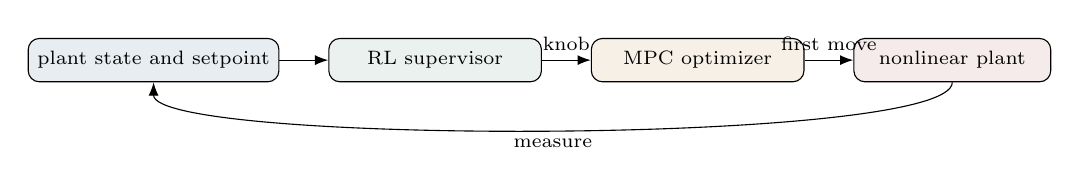
\begin{tikzpicture}[node distance=0.62cm, >=Latex, every node/.style={font=\scriptsize}]
\node[draw,rounded corners,fill=maccblue!10,minimum width=2.6cm,minimum height=0.55cm] (obs) {plant state and setpoint};
\node[draw,rounded corners,fill=maccgreen!10,right=of obs,minimum width=2.7cm,minimum height=0.55cm] (rl) {RL supervisor};
\node[draw,rounded corners,fill=maccgold!12,right=of rl,minimum width=2.7cm,minimum height=0.55cm] (mpc) {MPC optimizer};
\node[draw,rounded corners,fill=maccred!10,right=of mpc,minimum width=2.5cm,minimum height=0.55cm] (plant) {nonlinear plant};
\draw[->] (obs) -- (rl);
\draw[->] (rl) -- node[above]{knob} (mpc);
\draw[->] (mpc) -- node[above]{first move} (plant);
\draw[->] (plant.south) .. controls +(0,-0.8) and +(0,-0.8) .. node[below]{measure} (obs.south);
\end{tikzpicture}
\end{center}

\takeawaybox{RL learns which MPC design knob to change while MPC remains the constrained move generator.}
\end{frame}

%============================= Slide 3 ============================
\begin{frame}
\frametitle{\large \textbf{Common notation for all supervisors}}
\scriptsize

\begin{columns}[T,onlytextwidth]
\begin{column}{0.47\textwidth}
\begin{block}{Plant and estimator coordinates}
\begin{align*}
x_{a,k+1} &= A_{\mathrm{aug}}x_{a,k}+B_{\mathrm{aug}}\Delta u_k,\\
y_k &= C_{\mathrm{aug}}x_{a,k},\\
\hat{x}_{a,k+1} &= A_{\mathrm{aug}}\hat{x}_{a,k}
+B_{\mathrm{aug}}\Delta u_k+L(y_k-\hat{y}_k).
\end{align*}
\vspace{-0.15cm}
\begin{itemize}\justifying
  \setlength\itemsep{0.3ex}
  \item \(x_a\) is the augmented offset-free state.
  \item \(u\) is manipulated input and \(\Delta u_k=u_k-u_{k-1}\).
  \item \(y\) is controlled output.
  \item Calculations use scaled deviation variables unless marked physical.
\end{itemize}
\end{block}
\end{column}

\begin{column}{0.51\textwidth}
\begin{block}{Receding-horizon MPC objective}
\begin{align*}
J_k &= \sum_{i=1}^{N_p} e_{k+i}^{\top}Qe_{k+i}
+\sum_{i=0}^{N_c-1}\Delta u_{k+i}^{\top}R\Delta u_{k+i},\\
e_{k+i} &= y_{k+i}-y^{\mathrm{sp}}_{k+i},\\
\Delta U_k^\star &= \arg\min_{\Delta U_k} J_k
\quad \mathrm{s.t.}\quad u_{\min}\le u_{k+i}\le u_{\max}.
\end{align*}
\vspace{-0.15cm}
\begin{itemize}\justifying
  \setlength\itemsep{0.3ex}
  \item \(N_p\) is prediction horizon.
  \item \(N_c\) is control horizon.
  \item Only the first optimized move is applied.
\end{itemize}
\end{block}
\end{column}
\end{columns}

\takeawaybox{Every RL method changes a different term in this same MPC loop.}
\end{frame}

%============================= Slide 4 ============================
\begin{frame}
\frametitle{\large \textbf{The algorithm families are different ways to change MPC}}
\scriptsize

\begin{center}
\tiny
\renewcommand{\arraystretch}{1.25}
\begin{tabular}{p{0.19\textwidth}p{0.23\textwidth}p{0.25\textwidth}p{0.21\textwidth}}
\toprule
\textbf{Family} & \textbf{RL action} & \textbf{MPC quantity changed} & \textbf{Typical agent}\\
\midrule
Horizon & discrete recipe index & \(N_p,N_c\) & DQN or dueling DQN\\
Weights & four continuous multipliers & \(Q,R\) penalties & TD3, SAC, SG-TD3\\
Residual & continuous correction in input space & final input after MPC & TD3, SAC, TD7, SG-TD3\\
Dynamic matrix & continuous correction vector \(z\) & Markov blocks \(M_i\) and lifted matrix \(G\) & TD3, SG-TD3\\
Combined & multiple actions & horizon, weights, model, residual & multi-agent supervisor\\
\bottomrule
\end{tabular}
\end{center}

\vspace{0.05cm}
\begin{block}{Two process settings}
\begin{itemize}\justifying
  \setlength\itemsep{0.25ex}
  \item Polymer CSTR: controlled outputs \((\eta,T)\), manipulated inputs \((Q_c,Q_m)\).
  \item Distillation column: tray-24 ethane composition and tray-85 temperature, manipulated inputs reflux flow and reboiler duty.
\end{itemize}
\end{block}

\takeawaybox{The methods are interpretable because each action coordinate has a controller meaning.}
\end{frame}

%============================= Slide 5 ============================
\begin{frame}
\frametitle{\large \textbf{Learning signal: the agent sees closed-loop reward, not only one-step error}}
\scriptsize

\begin{block}{Generic reward form}
\begin{align*}
r_k &=
- e_k^{\top}Q_r e_k
- \Delta u_k^{\top}R_r\Delta u_k
+ b_{\mathrm{near}}(e_k)
- p_{\mathrm{viol}}(k),\\
G_t &= \sum_{\ell=0}^{\infty}\gamma^\ell r_{t+\ell}.
\end{align*}
\end{block}

\begin{columns}[T,onlytextwidth]
\begin{column}{0.49\textwidth}
\begin{block}{What the reward encourages}
\begin{itemize}\justifying
  \setlength\itemsep{0.25ex}
  \item small output tracking error
  \item reasonable input movement
  \item staying near target bands
\end{itemize}
\end{block}
\end{column}
\begin{column}{0.49\textwidth}
\begin{block}{What it does not guarantee by itself}
\begin{itemize}\justifying
  \setlength\itemsep{0.25ex}
  \item no hard safety certificate
  \item no guaranteed constraint satisfaction for raw actor output
  \item no guarantee that short-term prediction score matches long-term return
\end{itemize}
\end{block}
\end{column}
\end{columns}

\takeawaybox{Reward defines the learning objective, while MPC and safety gates define the executable controller envelope.}
\end{frame}

%============================= Slide 6 ============================
\begin{frame}
\frametitle{\large \textbf{Horizon supervisor: RL changes how far MPC looks ahead}}
\scriptsize

\begin{columns}[T,onlytextwidth]
\begin{column}{0.48\textwidth}
\begin{block}{Discrete action table}
\begin{align*}
\mathcal{A}_H
&=\{(N_p^{(j)},N_c^{(j)}):N_c^{(j)}\le N_p^{(j)}\},\\
a_k&=j,\qquad (N_p,N_c)_k=\mathcal{A}_H[j].
\end{align*}
\vspace{-0.12cm}
\begin{itemize}\justifying
  \setlength\itemsep{0.35ex}
  \item Polymer grid: \(N_p\in\{8,\ldots,19\}\), \(N_c\in\{3,\ldots,9\}\).
  \item Distillation grid: \(N_p\in\{4,\ldots,14\}\), \(N_c\in\{2,\ldots,13\}\).
  \item Invalid choices with \(N_c>N_p\) are removed.
\end{itemize}
\end{block}
\end{column}

\begin{column}{0.50\textwidth}
\begin{block}{Why horizon matters}
\begin{itemize}\justifying
  \setlength\itemsep{0.45ex}
  \item Larger \(N_p\): sees slower settling and delayed effects.
  \item Smaller \(N_p\): cheaper optimization and more local behavior.
  \item Larger \(N_c\): gives MPC more move-shaping freedom.
  \item Smaller \(N_c\): makes input plans simpler and usually smoother.
  \item DQN is natural because the action is a finite recipe index.
\end{itemize}
\end{block}
\end{column}
\end{columns}

\begin{center}
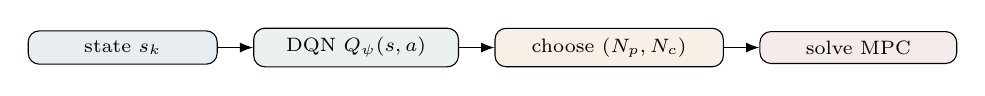
\begin{tikzpicture}[>=Latex, node distance=0.45cm, every node/.style={font=\scriptsize}]
\node[draw,rounded corners,fill=maccblue!10,minimum width=2.4cm] (s) {state \(s_k\)};
\node[draw,rounded corners,fill=maccgreen!10,right=of s,minimum width=2.6cm] (q) {DQN \(Q_\psi(s,a)\)};
\node[draw,rounded corners,fill=maccgold!12,right=of q,minimum width=2.9cm] (a) {choose \((N_p,N_c)\)};
\node[draw,rounded corners,fill=maccred!10,right=of a,minimum width=2.5cm] (m) {solve MPC};
\draw[->] (s) -- (q);
\draw[->] (q) -- (a);
\draw[->] (a) -- (m);
\end{tikzpicture}
\end{center}

\takeawaybox{The horizon agent changes the time scale of MPC, not the plant input directly.}
\end{frame}

%============================= Slide 7 ============================
\begin{frame}
\frametitle{\large \textbf{Horizon mathematics: DQN learns a value for each horizon recipe}}
\scriptsize

\begin{block}{Action-value learning}
\begin{align*}
Q_\psi(s_k,a_k)
&\approx \mathbb{E}\left[\sum_{\ell=0}^{\infty}\gamma^\ell r_{k+\ell}\mid s_k,a_k\right],\\
y_k^{\mathrm{DQN}}
&= r_k+\gamma(1-d_k)\max_{a'} Q_{\bar{\psi}}(s_{k+1},a'),\\
\mathcal{L}_{Q}
&= \mathbb{E}_{(s,a,r,s')\sim\mathcal{D}}
\left[\left(Q_\psi(s,a)-y^{\mathrm{DQN}}\right)^2\right].
\end{align*}
\end{block}

\begin{block}{Decision rule}
\begin{align*}
a_k =
\begin{cases}
\mathrm{random}(\mathcal{A}_H), & \mathrm{with}\ \epsilon_k,\\
\arg\max_a Q_\psi(s_k,a), & \mathrm{otherwise}.
\end{cases}
\end{align*}
Epsilon decays so early training explores horizons and late training exploits learned recipes.
\end{block}

\end{frame}

%============================= Slide 8 ============================
\begin{frame}
\frametitle{\large \textbf{Dueling DQN separates state difficulty from action preference}}
\scriptsize

\begin{block}{Dueling horizon value decomposition}
\begin{align*}
Q_\psi(s,a)
&=V_\psi(s)+A_\psi(s,a)
-\frac{1}{|\mathcal{A}_H|}\sum_{a'\in\mathcal{A}_H}A_\psi(s,a').
\end{align*}
\end{block}

\begin{columns}[T,onlytextwidth]
\begin{column}{0.49\textwidth}
\begin{block}{State-value stream}
\begin{itemize}\justifying
  \setlength\itemsep{0.35ex}
  \item learns whether the current process condition is easy or difficult
  \item does not need to explain differences between horizon actions
\end{itemize}
\end{block}
\end{column}

\begin{column}{0.49\textwidth}
\begin{block}{Advantage stream}
\begin{itemize}\justifying
  \setlength\itemsep{0.35ex}
  \item learns which horizon recipe is better in the current state
  \item helps when many recipes have similar absolute return
\end{itemize}
\end{block}
\end{column}
\end{columns}

\takeawaybox{Dueling DQN is useful when horizon choices are close in value but still different in closed-loop behavior.}
\end{frame}

%============================= Slide 9 ============================
\begin{frame}
\frametitle{\large \textbf{Weight supervisor: RL changes the tradeoff inside MPC}}
\scriptsize

\begin{block}{Nominal and adapted objectives}
\vspace{-0.1cm}
\begin{align*}
J_0 &= \sum_{i=1}^{N_p} e_i^\top Q_0 e_i
+\sum_{i=0}^{N_c-1}\Delta u_i^\top R_0\Delta u_i,\\
Q(a_k) &= \diag(w_{Q,k})Q_0,\qquad
R(a_k)=\diag(w_{R,k})R_0,\\
J(a_k)&=\sum_{i=1}^{N_p} e_i^\top Q(a_k)e_i
+\sum_{i=0}^{N_c-1}\Delta u_i^\top R(a_k)\Delta u_i.
\end{align*}
\vspace{-0.2cm}
\end{block}

\begin{block}{Control interpretation}
Larger \(w_{Q_i}\) makes MPC track output \(i\) more aggressively. Larger \(w_{R_j}\) makes MPC move input \(j\) more smoothly. Typical multiplier bounds are \(0.75\le w_i\le 2.0\).
\end{block}

\takeawaybox{Weight adaptation is a tuning policy: the model stays fixed and RL changes controller aggressiveness.}
\end{frame}

%============================= Slide 9 ============================
\begin{frame}
\frametitle{\large \textbf{Weight algorithm: identity is the safe supervisor}}
\scriptsize

\begin{center}
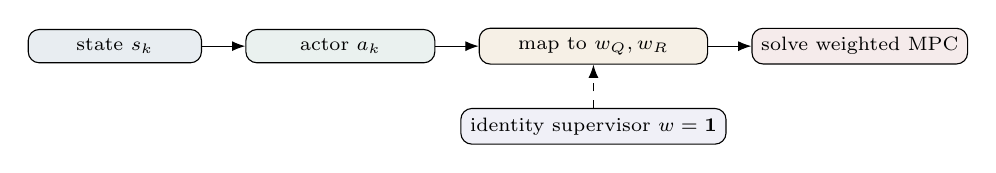
\begin{tikzpicture}[>=Latex, node distance=0.55cm, every node/.style={font=\scriptsize}]
\node[draw,rounded corners,fill=maccblue!10,minimum width=2.2cm] (s) {state \(s_k\)};
\node[draw,rounded corners,fill=maccgreen!10,right=of s,minimum width=2.4cm] (actor) {actor \(a_k\)};
\node[draw,rounded corners,fill=maccgold!12,right=of actor,minimum width=2.9cm] (map) {map to \(w_Q,w_R\)};
\node[draw,rounded corners,fill=maccred!10,right=of map,minimum width=2.5cm] (mpc) {solve weighted MPC};
\draw[->] (s) -- (actor);
\draw[->] (actor) -- (map);
\draw[->] (map) -- (mpc);
\node[draw,rounded corners,fill=lightgray,below=0.55cm of map,minimum width=2.7cm] (id) {identity supervisor \(w=\mathbf{1}\)};
\draw[->,dashed] (id) -- (map);
\end{tikzpicture}
\end{center}

\begin{columns}[T,onlytextwidth]
\begin{column}{0.50\textwidth}
\begin{block}{Training transition}
\begin{align*}
s_k &\rightarrow a_k \rightarrow (Q_k,R_k)
\rightarrow \Delta u_k^\star \rightarrow y_{k+1},\\
\mathcal{D}&\leftarrow(s_k,a_k^{\mathrm{exec}},r_k,s_{k+1},d_k).
\end{align*}
Replay stores the executed multiplier action so the critic learns the action that actually produced the next state.
\end{block}
\end{column}

\begin{column}{0.48\textwidth}
\begin{block}{Safety role}
\begin{itemize}\justifying
  \setlength\itemsep{0.4ex}
  \item Identity action recovers nominal MPC weights.
  \item Nonfinite multipliers or failed solves can fall back to identity.
  \item SG-TD3 can compare actor weights against identity weights using the same critics.
\end{itemize}
\end{block}
\end{column}
\end{columns}

\takeawaybox{For weights, safety means the controller can always fall back to familiar fixed tuning.}
\end{frame}

%============================= Slide 10 ============================
\begin{frame}
\frametitle{\large \textbf{Residual supervisor: RL adds a bounded correction after MPC}}
\scriptsize

\begin{block}{Residual correction around nominal MPC}
\begin{align*}
\Delta u_k^{\mathrm{mpc}} &= \mathrm{MPC}(s_k,y_k^{\mathrm{sp}}),\\
\delta u_k^{\mathrm{res}} &= \delta_{\min}
+\frac{a_k+1}{2}\odot(\delta_{\max}-\delta_{\min}),\\
\Delta u_k^{\mathrm{exec}} &= \clip\!\left(
\Delta u_k^{\mathrm{mpc}}+\rho_k\,\delta u_k^{\mathrm{res}},
\Delta u_{\min},\Delta u_{\max}
\right).
\end{align*}
\end{block}

\begin{columns}[T,onlytextwidth]
\begin{column}{0.47\textwidth}
\begin{block}{Meaning of each term}
\begin{itemize}\justifying
  \setlength\itemsep{0.35ex}
  \item \(\Delta u^{\mathrm{mpc}}\): stabilizing baseline move.
  \item \(\delta u^{\mathrm{res}}\): learned local correction.
  \item \(\rho_k\): optional authority factor.
  \item Clipping enforces input or move limits.
\end{itemize}
\end{block}
\end{column}

\begin{column}{0.51\textwidth}
\begin{block}{Typical correction bounds}
\begin{itemize}\justifying
  \setlength\itemsep{0.35ex}
  \item Polymer residual action: roughly \([-0.25,0.25]^2\) in scaled move coordinates.
  \item Distillation residual action: roughly \([-0.02,0.02]^2\).
  \item The correction is intentionally smaller than direct input authority.
\end{itemize}
\end{block}
\end{column}
\end{columns}

\takeawaybox{Residual RL is local adaptation: MPC supplies the main move and RL repairs what MPC misses.}
\end{frame}

%============================= Slide 11 ============================
\begin{frame}
\frametitle{\large \textbf{Residual safety: zero residual is the natural fallback}}
\scriptsize

\begin{center}
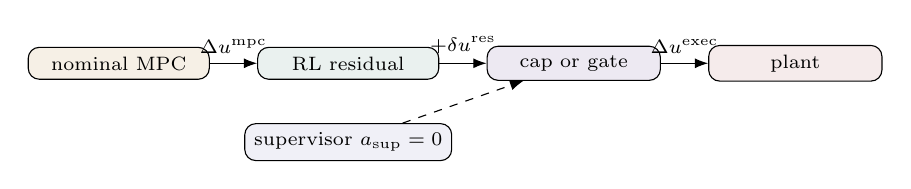
\begin{tikzpicture}[>=Latex, node distance=0.6cm, every node/.style={font=\scriptsize}]
\node[draw,rounded corners,fill=maccgold!12,minimum width=2.3cm] (mpc) {nominal MPC};
\node[draw,rounded corners,fill=maccgreen!10,right=of mpc,minimum width=2.3cm] (actor) {RL residual};
\node[draw,rounded corners,fill=maccpurple!12,right=of actor,minimum width=2.2cm] (gate) {cap or gate};
\node[draw,rounded corners,fill=maccred!10,right=of gate,minimum width=2.2cm] (plant) {plant};
\draw[->] (mpc) -- node[above]{\(\Delta u^{\mathrm{mpc}}\)} (actor);
\draw[->] (actor) -- node[above]{\(+\delta u^{\mathrm{res}}\)} (gate);
\draw[->] (gate) -- node[above]{\(\Delta u^{\mathrm{exec}}\)} (plant);
\node[draw,rounded corners,fill=lightgray,below=0.55cm of actor,minimum width=2.4cm] (zero) {supervisor \(a_{\mathrm{sup}}=0\)};
\draw[->,dashed] (zero) -- (gate);
\end{tikzpicture}
\end{center}

\begin{columns}[T,onlytextwidth]
\begin{column}{0.49\textwidth}
\begin{block}{Authority scheduling}
\begin{align*}
\rho_k &= \rho_{\min}+(1-\rho_{\min})g_k,\\
g_k&\in[0,1].
\end{align*}
The schedule can release authority gradually after warm start, or use a mismatch confidence signal.
\end{block}
\end{column}

\begin{column}{0.49\textwidth}
\begin{block}{Guard logic}
\begin{itemize}\justifying
  \setlength\itemsep{0.35ex}
  \item zero residual gives nominal MPC
  \item early-release guard can shrink the residual
  \item nonfinite output falls back to zero residual
  \item replay stores the residual that was actually executed
\end{itemize}
\end{block}
\end{column}
\end{columns}

\takeawaybox{The residual family has a built-in safe action: do nothing beyond MPC.}
\end{frame}

%============================= Slide 12 ============================
\begin{frame}
\frametitle{\large \textbf{Dynamic-matrix supervisor: Markov parameters are the prediction model}}
\scriptsize

\begin{block}{Impulse-response or Markov blocks}
\begin{align*}
M_i &= C_{\mathrm{aug}}A_{\mathrm{aug}}^{i-1}B_{\mathrm{aug}},
\qquad i=1,\ldots,N_p,\\
M_i &\in \R^{n_y\times n_u}.
\end{align*}
\vspace{-0.15cm}
\begin{itemize}\justifying
  \setlength\itemsep{0.35ex}
  \item \(M_i\) maps an input move at the current time to output response \(i\) samples later.
  \item In classical control language, the lifted matrix made from \(M_i\) is the dynamic matrix.
  \item In the code this is the Markov correction path.
\end{itemize}
\end{block}

\begin{center}
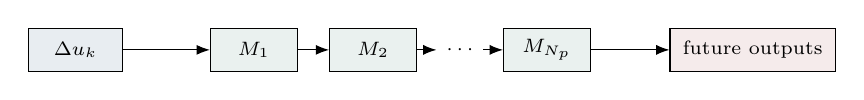
\begin{tikzpicture}[>=Latex, every node/.style={font=\scriptsize}]
\node[draw,fill=maccblue!10,minimum width=1.2cm,minimum height=0.55cm] (du) {\(\Delta u_k\)};
\node[draw,fill=maccgreen!10,right=1.1cm of du,minimum width=1.1cm,minimum height=0.55cm] (m1) {\(M_1\)};
\node[draw,fill=maccgreen!10,right=0.4cm of m1,minimum width=1.1cm,minimum height=0.55cm] (m2) {\(M_2\)};
\node[right=0.25cm of m2] (dots) {\(\cdots\)};
\node[draw,fill=maccgreen!10,right=0.25cm of dots,minimum width=1.1cm,minimum height=0.55cm] (mp) {\(M_{N_p}\)};
\node[draw,fill=maccred!10,right=1.0cm of mp,minimum width=2.1cm,minimum height=0.55cm] (y) {future outputs};
\draw[->] (du) -- (m1);
\draw[->] (m1) -- (m2);
\draw[->] (mp) -- (y);
\draw[->] (m2) -- (dots);
\draw[->] (dots) -- (mp);
\end{tikzpicture}
\end{center}

\takeawaybox{\(M_i\) is not a neural-network parameter. It is a physical lifted-response coefficient used by MPC.}
\end{frame}

%============================= Slide 13 ============================
\begin{frame}
\frametitle{\large \textbf{Dynamic matrix \(G\): stacking Markov blocks gives lifted prediction}}
\scriptsize

\begin{block}{Lifted prediction equation}
\begin{align*}
Y_k &= Y_k^{\mathrm{free}} + G_0 \Delta U_k,\\
Y_k &= \begin{bmatrix}y_{k+1}\\y_{k+2}\\ \vdots\\ y_{k+N_p}\end{bmatrix},
\qquad
\Delta U_k=\begin{bmatrix}\Delta u_k\\\Delta u_{k+1}\\ \vdots\\ \Delta u_{k+N_c-1}\end{bmatrix}.
\end{align*}
\end{block}

\begin{block}{Why this form matters}
\begin{itemize}\justifying
  \setlength\itemsep{0.35ex}
  \item \(Y^{\mathrm{free}}\) is the output response from the current estimated state with no new input moves.
  \item \(G_0\Delta U\) is the future output contribution caused by planned input moves.
  \item Changing \(G\) changes how MPC believes each move will affect future outputs.
\end{itemize}
\end{block}

\takeawaybox{The Markov method adapts the matrix that converts planned input moves into predicted output trajectories.}
\end{frame}

%============================= Slide 14 ============================
\begin{frame}
\frametitle{\large \textbf{The dynamic matrix is a block-Toeplitz matrix}}
\scriptsize

\begin{align*}
G_0 =
\begin{bmatrix}
M_1 & 0 & 0 & \cdots & 0\\
M_2 & M_1 & 0 & \cdots & 0\\
M_3 & M_2 & M_1 & \cdots & 0\\
\vdots & \vdots & \vdots & \ddots & \vdots\\
M_{N_p} & M_{N_p-1} & M_{N_p-2} & \cdots & M_{N_p-N_c+1}
\end{bmatrix}.
\end{align*}

\begin{block}{Reading one block column}
The first block column tells how the current move \(\Delta u_k\) affects all future outputs. The second block column tells how the next planned move \(\Delta u_{k+1}\) affects outputs one sample later, and so on.
\end{block}

\begin{block}{Why MPC likes this structure}
The entire prediction over \(N_p\) samples becomes one linear map from the planned move sequence \(\Delta U_k\) to the stacked output sequence \(Y_k\). This is why changing \(M_i\) changes the optimizer's future view.
\end{block}

\takeawaybox{The dynamic matrix is the finite-horizon input-output model seen by MPC.}
\end{frame}

%============================= Slide 15 ============================
\begin{frame}
\frametitle{\large \textbf{What is \(z\)? A bounded correction coordinate for the dynamic matrix}}
\scriptsize

\begin{block}{Basis expansion of Markov blocks}
\begin{align*}
M_i(z_k) &= M_{i,0}+\sum_{j=1}^{r}z_{j,k}B_i^{(j)},\\
G(z_k) &= \Toeplitz\left(M_1(z_k),\ldots,M_{N_p}(z_k)\right),\\
z_k &\in[-z_{\max},z_{\max}]^r.
\end{align*}
\end{block}

\begin{block}{Meaning of \(z_j\)}
\begin{itemize}\justifying
  \setlength\itemsep{0.35ex}
  \item \(z_j=0\): nominal dynamic matrix.
  \item \(z_j>0\): strengthen the selected basis direction.
  \item \(z_j<0\): weaken or reverse that basis direction.
  \item \(z_{\max}\) limits how far the model can move.
\end{itemize}
\end{block}

\takeawaybox{\(z\) is the RL or LS action in Markov space: it edits the prediction model, then MPC still computes the input.}
\end{frame}

%============================= Slide 15 ============================
\begin{frame}
\frametitle{\large \textbf{Least-squares Markov correction supplies a supervisor action}}
\scriptsize

\begin{block}{Online LS fit over a recent prediction window}
\begin{align*}
z_k^{\mathrm{LS}}
&=\arg\min_z
\sum_{\tau\in\mathcal{W}_k}
\norm{Y_\tau^{\mathrm{meas}}
-\left(Y_\tau^{\mathrm{free}}+G(z)\Delta U_\tau^{\mathrm{real}}\right)}_{W_y}^2
+\lambda_z\norm{z}_2^2,\\
\mathcal{W}_k&=\{\tau: \tau \ \mathrm{has}\ N_p\ \mathrm{future\ measurements}\}.
\end{align*}
\end{block}

\begin{block}{Prediction-improvement score}
\begin{align*}
S_{\mathrm{pred}}(z)
&=\sum_{\tau\in\mathcal{W}_k}
\left(
\norm{W_yE_0(\tau)}_2^2-\norm{W_yE_z(\tau)}_2^2
\right)
-\lambda_z\norm{z}_2^2,\\
E_0(\tau)&=Y_\tau^{\mathrm{meas}}-\left(Y_\tau^{\mathrm{free}}+G_0\Delta U_\tau^{\mathrm{real}}\right),\\
E_z(\tau)&=Y_\tau^{\mathrm{meas}}-\left(Y_\tau^{\mathrm{free}}+G(z)\Delta U_\tau^{\mathrm{real}}\right).
\end{align*}
\end{block}

\takeawaybox{LS is a data-driven local model correction, useful as teacher, fallback, or SG-TD3 supervisor.}
\end{frame}

%============================= Slide 16 ============================
\begin{frame}
\frametitle{\large \textbf{Markov TD3: the actor proposes \(z\), MPC executes with \(G(z)\)}}
\scriptsize

\begin{center}
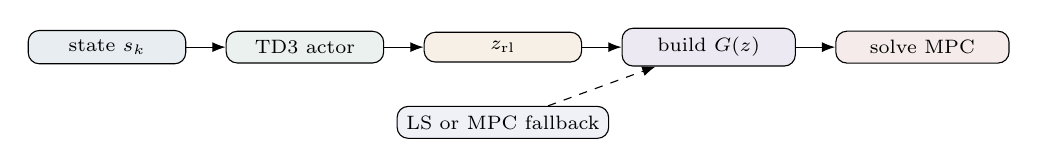
\begin{tikzpicture}[>=Latex, node distance=0.5cm, every node/.style={font=\scriptsize}]
\node[draw,rounded corners,fill=maccblue!10,minimum width=2.0cm] (s) {state \(s_k\)};
\node[draw,rounded corners,fill=maccgreen!10,right=of s,minimum width=2.0cm] (td3) {TD3 actor};
\node[draw,rounded corners,fill=maccgold!12,right=of td3,minimum width=2.0cm] (z) {\(z_{\mathrm{rl}}\)};
\node[draw,rounded corners,fill=maccpurple!12,right=of z,minimum width=2.2cm] (g) {build \(G(z)\)};
\node[draw,rounded corners,fill=maccred!10,right=of g,minimum width=2.2cm] (mpc) {solve MPC};
\draw[->] (s) -- (td3);
\draw[->] (td3) -- (z);
\draw[->] (z) -- (g);
\draw[->] (g) -- (mpc);
\node[draw,rounded corners,fill=lightgray,below=0.55cm of z,minimum width=2.2cm] (ls) {LS or MPC fallback};
\draw[->,dashed] (ls) -- (g);
\end{tikzpicture}
\end{center}

\begin{block}{Runtime candidate evaluation}
\begin{align*}
z_{\mathrm{rl}} &= z_{\max}\clip(a_{\mathrm{rl}},-1,1),\\
U_{\mathrm{rl}}^\star &= \arg\min_U J(U;G(z_{\mathrm{rl}})),\\
\mathrm{accept} &\Leftrightarrow
S_{\mathrm{pred}}(z_{\mathrm{rl}})>s_{\min}
\quad \mathrm{and}\quad
d_{\mathrm{gain}}(z_{\mathrm{rl}})\le d_{\max}
\quad \mathrm{and}\quad
\Delta J_{\mathrm{nom}}\le \epsilon.
\end{align*}
\end{block}

\begin{itemize}\justifying
  \setlength\itemsep{0.3ex}
  \item Guarded Markov TD3 can execute TD3, fall back to LS, or fall back to nominal MPC.
  \item The SG-TD3 Markov wrapper uses LS-or-MPC as the supervisor during warm start and critic warm.
\end{itemize}

\takeawaybox{Markov control learns a model-correction action, then relies on MPC to translate that model into inputs.}
\end{frame}

%============================= Slide 17 ============================
\begin{frame}
\frametitle{\large \textbf{Standard TD3 is the continuous-control base agent}}
\scriptsize

\begin{columns}[T,onlytextwidth]
\begin{column}{0.50\textwidth}
\begin{block}{Actor and twin critics}
\begin{align*}
a_k &= \mu_\theta(s_k)+\eta_k,\\
Q_{\phi_1}(s,a),\quad Q_{\phi_2}(s,a).
\end{align*}
The actor proposes a normalized action. The critics estimate expected return for state-action pairs.
\end{block}

\begin{block}{Target-policy smoothing}
\begin{align*}
\tilde{a}_{k+1}
&=\clip\left(\mu_{\bar{\theta}}(s_{k+1})+\epsilon,\ -a_{\max},a_{\max}\right).
\end{align*}
\end{block}
\end{column}

\begin{column}{0.48\textwidth}
\begin{block}{Critic and actor losses}
\begin{align*}
y_k &= r_k+\gamma(1-d_k)
\min_{i=1,2}Q_{\bar{\phi}_i}(s_{k+1},\tilde{a}_{k+1}),\\
\mathcal{L}_{Q_i}
&=\mathbb{E}\left[(Q_{\phi_i}(s_k,a_k)-y_k)^2\right],\\
\mathcal{L}_{\pi}
&=-\mathbb{E}\left[Q_{\phi_1}(s_k,\mu_\theta(s_k))\right].
\end{align*}
\end{block}

\begin{block}{TD3 protections}
\begin{itemize}\justifying
  \setlength\itemsep{0.35ex}
  \item clipped double-Q target reduces overestimation
  \item delayed actor update stabilizes critic learning
  \item target noise smooths sharp critic errors
\end{itemize}
\end{block}
\end{column}
\end{columns}

\takeawaybox{TD3 stabilizes continuous action learning, but it still executes only the actor candidate unless we add a supervisor gate.}
\end{frame}

%============================= Slide 18 ============================
\begin{frame}
\frametitle{\large \textbf{SG-TD3 adds a second candidate action before execution}}
\scriptsize

\begin{block}{Two candidates in the same normalized action space}
\begin{align*}
a_{\mathrm{rl},k} &= \mu_\theta(s_k),\\
a_{\mathrm{sup},k} &= \mu_{\mathrm{sup}}(s_k),\\
a_{\mathrm{rl},k},a_{\mathrm{sup},k}&\in[-a_{\max},a_{\max}]^{n_a}.
\end{align*}
\end{block}

\begin{center}
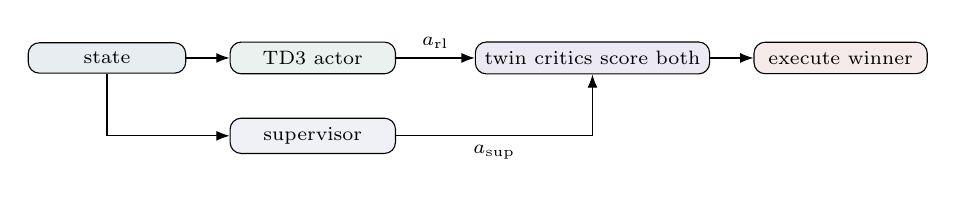
\begin{tikzpicture}[>=Latex, node distance=0.55cm, every node/.style={font=\scriptsize}]
\node[draw,rounded corners,fill=maccblue!10,minimum width=2.0cm] (s) {state};
\node[draw,rounded corners,fill=maccgreen!10,right=of s,minimum width=2.1cm] (actor) {TD3 actor};
\node[draw,rounded corners,fill=lightgray,below=0.55cm of actor,minimum width=2.1cm] (sup) {supervisor};
\node[draw,rounded corners,fill=maccpurple!12,right=1.0cm of actor,minimum width=2.4cm] (critics) {twin critics score both};
\node[draw,rounded corners,fill=maccred!10,right=of critics,minimum width=2.2cm] (exec) {execute winner};
\draw[->] (s) -- (actor);
\draw[->] (s) |- (sup);
\draw[->] (actor) -- node[above]{\(a_{\mathrm{rl}}\)} (critics);
\draw[->] (sup) -| node[pos=0.25,below]{\(a_{\mathrm{sup}}\)} (critics);
\draw[->] (critics) -- (exec);
\end{tikzpicture}
\end{center}

\begin{block}{Execution difference from standard TD3}
Standard TD3 executes \(a_{\mathrm{rl}}\) whenever the policy is live. SG-TD3 evaluates \(a_{\mathrm{rl}}\) against \(a_{\mathrm{sup}}\) first, then executes the selected candidate and stores that executed action in replay.
\end{block}

\end{frame}

%============================= Slide 19 ============================
\begin{frame}
\frametitle{\large \textbf{SG-TD3 scoring: critic value minus uncertainty and motion penalties}}
\scriptsize

\begin{block}{Conservative score used by the gate}
\begin{align*}
Q_{\min}(s,a)&=\min\left(Q_1(s,a),Q_2(s,a)\right),\\
D_Q(s,a)&=|Q_1(s,a)-Q_2(s,a)|,\\
S(s,a)&=Q_{\min}(s,a)
-\rho_QD_Q(s,a)
-\kappa_{\mathrm{prev}}\norm{a-a_{\mathrm{prev}}}_2^2
-\kappa_{\mathrm{sup}}\norm{a-a_{\mathrm{sup}}}_2^2.
\end{align*}
\end{block}

\begin{columns}[T,onlytextwidth]
\begin{column}{0.48\textwidth}
\begin{block}{Gate rule}
\begin{align*}
a_k^{\mathrm{exec}}=
\begin{cases}
a_{\mathrm{rl},k},&
S(s_k,a_{\mathrm{rl},k})>
S(s_k,a_{\mathrm{sup},k})+\epsilon_A,\\
a_{\mathrm{sup},k},&\mathrm{otherwise}.
\end{cases}
\end{align*}
\end{block}
\end{column}

\begin{column}{0.50\textwidth}
\begin{block}{Current critic-warm Markov settings}
\begin{itemize}\justifying
  \setlength\itemsep{0.35ex}
  \item \(\rho_Q=0.5\)
  \item \(\kappa_{\mathrm{sup}}=0.02\) for polymer Markov and new distillation Markov wrapper
  \item \(\kappa_{\mathrm{prev}}=0.01\)
  \item \(\epsilon_A=0\), default-to-supervisor on ties
\end{itemize}
\end{block}
\end{column}
\end{columns}

\takeawaybox{The gate rewards high value, penalizes critic disagreement, and avoids unnecessary jumps away from safe actions.}
\end{frame}

%============================= Slide 20 ============================
\begin{frame}
\frametitle{\large \textbf{SG-TD3 training: the critic learns executed actions}}
\scriptsize

\begin{block}{Replay stores the action that actually moved the plant}
\begin{align*}
\mathcal{D}\leftarrow
\left(s_k,a_k^{\mathrm{exec}},r_k,s_{k+1},d_k,
a_{\mathrm{rl},k},a_{\mathrm{sup},k},a_{\mathrm{prev},k},\mathrm{source}_k\right).
\end{align*}
\vspace{-0.18cm}
Counterfactual actor and supervisor actions are metadata. The critic sees the action that produced the next state.
\end{block}

\begin{block}{Critic target remains standard TD3}
\begin{align*}
y_k &= r_k+\gamma(1-d_k)
\min_i Q_{\bar{\phi}_i}(s_{k+1},\tilde{a}_{k+1}),\\
\mathcal{L}_{Q_i}
&=\mathbb{E}\left[(Q_{\phi_i}(s_k,a_k^{\mathrm{exec}})-y_k)^2\right].
\end{align*}
\end{block}

\takeawaybox{SG-TD3 improves safety through execution selection first, not by inventing counterfactual critic targets.}
\end{frame}

%============================= Slide 21 ============================
\begin{frame}
\frametitle{\large \textbf{SG-TD3 can also regularize the actor toward the supervisor}}
\scriptsize

\begin{block}{Optional supervisor-aware actor objective}
\begin{align*}
\mathcal{L}_\pi
&=-\mathbb{E}\left[Q_{\mathrm{mode}}(s,\mu_\theta(s))\right]
+\lambda_{\mathrm{sup}}\mathbb{E}\left[w_{\mathrm{sup}}\norm{\mu_\theta(s)-a_{\mathrm{sup}}}_2^2\right]
+\lambda_{\Delta a}\mathbb{E}\left[\norm{\mu_\theta(s)-a_{\mathrm{prev}}}_2^2\right],\\
w_{\mathrm{sup}}(s)
&=\sigma\left(\frac{\epsilon_A-\left[S(s,a_{\mathrm{rl}})-S(s,a_{\mathrm{sup}})\right]}{\tau_{\mathrm{sup}}}\right).
\end{align*}
\end{block}

\begin{block}{Interpretation}
\begin{itemize}\justifying
  \setlength\itemsep{0.35ex}
  \item \(w_{\mathrm{sup}}\) becomes large when the actor does not beat the supervisor by the margin.
  \item \(\lambda_{\mathrm{sup}}\) controls imitation pressure toward the supervisor.
  \item Current critic-warm wrappers use \(\lambda_{\mathrm{sup}}=0\), so this term is documented but disabled.
\end{itemize}
\end{block}

\takeawaybox{Actor regularization is optional. The current safety gain is mainly from the execution gate.}
\end{frame}

%============================= Slide 22 ============================
\begin{frame}
\frametitle{\large \textbf{Warm start and critic warm separate data collection from actor release}}
\scriptsize

\begin{center}
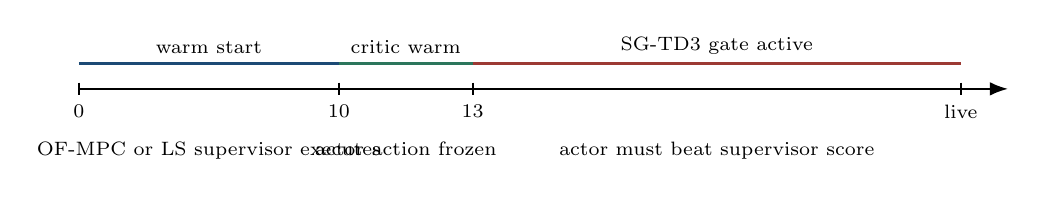
\begin{tikzpicture}[>=Latex, every node/.style={font=\scriptsize}]
\draw[thick,->] (0,0) -- (11.8,0);
\foreach \x/\lab in {0/0,3.3/10,5.0/13,11.2/live}
  \draw[thick] (\x,0.08) -- (\x,-0.08) node[below]{\lab};
\draw[very thick,maccblue] (0,0.32) -- (3.3,0.32);
\draw[very thick,maccgreen] (3.3,0.32) -- (5.0,0.32);
\draw[very thick,maccred] (5.0,0.32) -- (11.2,0.32);
\node[above] at (1.65,0.32) {warm start};
\node[above] at (4.15,0.32) {critic warm};
\node[above] at (8.1,0.32) {SG-TD3 gate active};
\node[below=0.55cm] at (1.65,0) {OF-MPC or LS supervisor executes};
\node[below=0.55cm] at (4.15,0) {actor action frozen};
\node[below=0.55cm] at (8.1,0) {actor must beat supervisor score};
\end{tikzpicture}
\end{center}

\vspace{0.15cm}

\begin{columns}[T,onlytextwidth]
\begin{column}{0.49\textwidth}
\begin{block}{Why warm start}
\begin{itemize}\justifying
  \setlength\itemsep{0.35ex}
  \item keeps early plant operation under OF-MPC or LS supervisor
  \item fills replay with meaningful closed-loop transitions
  \item prevents random actor actions from defining early process behavior
\end{itemize}
\end{block}
\end{column}

\begin{column}{0.49\textwidth}
\begin{block}{Why critic warm}
\begin{itemize}\justifying
  \setlength\itemsep{0.35ex}
  \item lets critics train before actor execution matters
  \item keeps the gate from trusting untrained Q-values too early
  \item mirrors the polymer Markov and new distillation Markov SG-TD3 design
\end{itemize}
\end{block}
\end{column}
\end{columns}

\takeawaybox{The schedule makes SG-TD3 a gradual release mechanism, not an immediate replacement for MPC.}
\end{frame}

%============================= Slide 22 ============================
\begin{frame}
\frametitle{\large \textbf{How SG-TD3 is adapted to each method family}}
\scriptsize

\begin{center}
\tiny
\renewcommand{\arraystretch}{1.18}
\begin{tabular}{p{0.15\textwidth}p{0.25\textwidth}p{0.24\textwidth}p{0.25\textwidth}}
\toprule
\textbf{Family} & \textbf{Actor action} & \textbf{Supervisor action} & \textbf{Safety benefit}\\
\midrule
Weights &
\(a_{\mathrm{rl}}\mapsto [w_Q,w_R]\) &
\(a_{\mathrm{sup}}\mapsto \mathbf{1}\) &
Actor must beat nominal fixed tuning before it changes aggressiveness\\
\addlinespace
Residual &
\(a_{\mathrm{rl}}\mapsto \delta u^{\mathrm{res}}\) &
\(a_{\mathrm{sup}}=0\) &
Actor must beat nominal-MPC residual before adding correction\\
\addlinespace
Markov &
\(a_{\mathrm{rl}}\mapsto z_{\mathrm{rl}}\) &
\(a_{\mathrm{sup}}\mapsto z_{\mathrm{LS}}\) if LS accepted, otherwise \(z=0\) &
Actor must beat local model correction or nominal dynamic matrix\\
\bottomrule
\end{tabular}
\end{center}

\vspace{0.1cm}

\begin{block}{Important distinction}
SG-TD3 is not a stability proof. It improves operational safety by changing execution, using supervisor-default ties, preserving fallback actions, and logging source fractions.
\end{block}

\takeawaybox{The same gate becomes method-specific because the supervisor action has a different control meaning in each family.}
\end{frame}

%============================= Slide 23 ============================
\begin{frame}
\frametitle{\large \textbf{Safety layers have different jobs}}
\scriptsize

\begin{center}
\tiny
\renewcommand{\arraystretch}{1.2}
\begin{tabular}{p{0.22\textwidth}p{0.31\textwidth}p{0.32\textwidth}}
\toprule
\textbf{Layer} & \textbf{What it protects} & \textbf{Typical effect}\\
\midrule
MPC constraints & physical input bounds and feasible moves & hard limits on optimized input\\
Warm start & early learning under weak replay & OF-MPC or LS executes first\\
Authority ramp & sudden post-warm actor release & gradually increases correction size\\
Fallback action & failed solve or nonfinite action & identity, zero residual, LS, or nominal MPC\\
SG-TD3 gate & weak critic evidence for actor action & supervisor wins unless actor proves value\\
Shadow diagnostics & audit without intervention & logs what safety layer would have done\\
\bottomrule
\end{tabular}
\end{center}

\vspace{0.05cm}
\begin{block}{Why the latest Markov wrapper turns live manual layers off}
The new distillation Markov SG-TD3 critic-warm runner disables live manual safety layers to isolate gate behavior. Shadow diagnostics stay on, so projected or rejected behavior can be audited without changing \(z_{\mathrm{exec}}\).
\end{block}

\takeawaybox{Safety is not one switch. It is a hierarchy of constraint handling, release scheduling, fallback, gating, and audit logs.}
\end{frame}

%============================= Slide 24 ============================
\begin{frame}
\frametitle{\large \textbf{Putting the algorithms side by side}}
\scriptsize

\begin{center}
\tiny
\renewcommand{\arraystretch}{1.18}
\begin{tabular}{p{0.15\textwidth}p{0.21\textwidth}p{0.21\textwidth}p{0.25\textwidth}}
\toprule
\textbf{Method} & \textbf{Changed object} & \textbf{Action dimension} & \textbf{Default safe action}\\
\midrule
Horizon & \(N_p,N_c\) & number of valid recipes & baseline horizon recipe\\
Weights & \(Q,R\) & \(4\) & \(w=\mathbf{1}\)\\
Residual & final \(\Delta u\) & \(n_u\) & \(\delta u=0\)\\
Dynamic matrix & \(G(z)\) through \(M_i(z)\) & basis size \(r\) & \(z=0\) or \(z^{\mathrm{LS}}\)\\
Combined & several MPC knobs & mixed discrete and continuous & per-agent fallback\\
\bottomrule
\end{tabular}
\end{center}

\vspace{0.1cm}

\begin{block}{Development path so far}
\begin{enumerate}\justifying
  \setlength\itemsep{0.35ex}
  \item Start with offset-free MPC as the baseline controller.
  \item Add one RL supervisor at a time: horizons, weights, residuals, matrix, dynamic matrix.
  \item Observe where standard TD3 is too aggressive or too suppressed by fallback.
  \item Add SG-TD3 so the actor competes with a meaningful supervisor action.
  \item Use critic-warm release and shadow diagnostics to separate learning from intervention.
\end{enumerate}
\end{block}

\takeawaybox{The project is moving from hand-built safety wrappers toward critic-based supervisor selection.}
\end{frame}

%============================= Slide 25 ============================
\begin{frame}
\frametitle{\large \textbf{Why SG-TD3 helps safety, and what remains uncertain}}
\scriptsize

\begin{columns}[T,onlytextwidth]
\begin{column}{0.49\textwidth}
\begin{block}{Safety improvements}
\begin{itemize}\justifying
  \setlength\itemsep{0.45ex}
  \item Actor action is not automatically executed.
  \item Supervisor wins ties and low-confidence cases.
  \item Critic disagreement is explicitly penalized.
  \item Warm start and critic warm reduce early random intervention.
  \item Replay remains transition-correct because it stores executed action.
  \item Source logs expose how often actor, supervisor, and fallback are used.
\end{itemize}
\end{block}
\end{column}

\begin{column}{0.49\textwidth}
\begin{block}{Remaining scientific risks}
\begin{itemize}\justifying
  \setlength\itemsep{0.45ex}
  \item Critic scores can still be wrong under distribution shift.
  \item A conservative gate can under-release the actor.
  \item A permissive gate can execute poorly valued actions.
  \item Supervisor quality matters.
  \item Improved reward is not the same as guaranteed stability.
  \item Distillation remains more sensitive than polymer because of strong coupling and slow dynamics.
\end{itemize}
\end{block}
\end{column}
\end{columns}

\takeawaybox{SG-TD3 is a safer execution architecture, not a substitute for closed-loop validation.}
\end{frame}

%============================= Slide 26 ============================
\begin{frame}
\frametitle{\large \textbf{Key message}}
\scriptsize

\begin{block}{One controller, many adaptive knobs}
\justifying
The unifying controller is offset-free MPC. The learning problem is not to replace that controller, but to learn which MPC quantity should be adapted online: horizon, cost weights, final residual correction, or the dynamic matrix used for prediction.
\end{block}

\begin{block}{Why dynamic-matrix Markov correction is important}
\justifying
The Markov method edits \(M_i=C_{\mathrm{aug}}A_{\mathrm{aug}}^{i-1}B_{\mathrm{aug}}\), the finite-horizon response blocks that form \(G\). This gives the RL agent a model-adaptation action \(z\), while MPC still performs constrained input optimization.
\end{block}

\begin{block}{Why SG-TD3 is the current safety direction}
\justifying
SG-TD3 changes the TD3 execution rule from actor-only to actor-versus-supervisor. In weights, the supervisor is identity tuning. In residuals, it is zero residual. In Markov, it is LS-or-MPC \(z\). This directly connects safety to a meaningful control fallback.
\end{block}

\takeawaybox{The research direction is interpretable adaptive MPC with learned release, not black-box direct control.}
\end{frame}

%============================= Backup title ============================
\begin{frame}
\begin{center}
\Large \textbf{Backup Slides}\\[0.5cm]
\small Detailed equations and implementation notes
\end{center}
\end{frame}

%============================= Slide 28 ============================
\begin{frame}
\frametitle{\large \textbf{Backup: lifted MPC objective in compact form}}
\scriptsize

\begin{block}{Stacked variables}
\begin{align*}
Y &= Y^{\mathrm{free}}+G\Delta U,\\
E &= Y-Y^{\mathrm{sp}},\\
\Delta U &= [\Delta u_k^\top,\ldots,\Delta u_{k+N_c-1}^\top]^\top.
\end{align*}
\end{block}

\begin{block}{Quadratic program form}
\begin{align*}
J(\Delta U)
&=E^\top\bar{Q}E+\Delta U^\top\bar{R}\Delta U\\
&=(Y^{\mathrm{free}}+G\Delta U-Y^{\mathrm{sp}})^\top
\bar{Q}
(Y^{\mathrm{free}}+G\Delta U-Y^{\mathrm{sp}})
\Delta U^\top\bar{R}\Delta U.
\end{align*}
\end{block}

\begin{block}{Weight and dynamic-matrix methods inside the same equation}
\begin{itemize}\justifying
  \setlength\itemsep{0.35ex}
  \item Weight RL changes \(\bar{Q}\) and \(\bar{R}\).
  \item Markov RL changes \(G\).
  \item Horizon RL changes the dimensions of \(Y\), \(\Delta U\), \(\bar{Q}\), \(\bar{R}\), and \(G\).
\end{itemize}
\end{block}
\end{frame}

%============================= Slide 29 ============================
\begin{frame}
\frametitle{\large \textbf{Backup: raw action mapping}}
\scriptsize

\begin{center}
\renewcommand{\arraystretch}{1.25}
\begin{tabular}{p{0.18\textwidth}p{0.38\textwidth}p{0.32\textwidth}}
\toprule
\textbf{Family} & \textbf{Raw action mapping} & \textbf{Interpretation}\\
\midrule
Weights &
\(w=w_{\min}+\frac{a+1}{2}\odot(w_{\max}-w_{\min})\) &
positive cost multipliers\\
Residual &
\(\delta u=\delta_{\min}+\frac{a+1}{2}\odot(\delta_{\max}-\delta_{\min})\) &
bounded input correction\\
Markov &
\(z=z_{\max}\clip(a,-1,1)\) &
bounded dynamic-matrix correction\\
Horizon &
\((N_p,N_c)=\mathcal{A}_H[a]\) &
discrete recipe lookup\\
\bottomrule
\end{tabular}
\end{center}

\vspace{0.15cm}
\begin{block}{Why normalize actions}
\begin{itemize}\justifying
  \setlength\itemsep{0.35ex}
  \item Neural networks output actions in comparable normalized ranges.
  \item Controller-specific scaling happens after the actor.
  \item Bounds are explicit and easy to audit.
\end{itemize}
\end{block}
\end{frame}

%============================= Slide 30 ============================
\begin{frame}
\frametitle{\large \textbf{Backup: Markov basis examples}}
\scriptsize

\begin{columns}[T,onlytextwidth]
\begin{column}{0.32\textwidth}
\begin{block}{IO-pair gain}
\begin{align*}
B_i^{(p,q)} &= E_{p,q}\odot M_{i,0},\\
z_{p,q} &: \mathrm{gain\ of\ output}\ p\\
&\mathrm{from\ input}\ q.
\end{align*}
\end{block}
\end{column}
\begin{column}{0.32\textwidth}
\begin{block}{Input-channel gain}
\begin{align*}
B_i^{(q)} &= M_{i,0}D_q,\\
z_q &: \mathrm{gain\ of\ all}\\
&\mathrm{outputs\ from\ input}\ q.
\end{align*}
\end{block}
\end{column}
\begin{column}{0.32\textwidth}
\begin{block}{Delay-shift}
\begin{align*}
B_i &\approx M_{i+1,0}-M_{i,0},\\
z &: \mathrm{apparent\ response}\\
&\mathrm{timing\ correction}.
\end{align*}
\end{block}
\end{column}
\end{columns}

\vspace{0.15cm}
\begin{block}{Why basis design is safety-relevant}
The basis determines what model changes are possible. A small \(z\) bound is not enough if the basis direction itself creates harmful coupled gain changes.
\end{block}
\end{frame}

%============================= Slide 31 ============================
\begin{frame}
\frametitle{\large \textbf{Backup: Markov candidate hierarchy}}
\scriptsize

\begin{center}
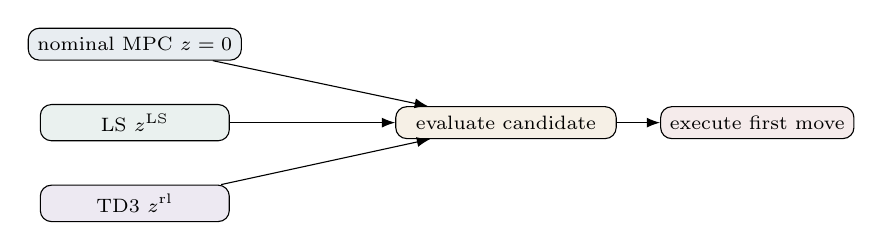
\begin{tikzpicture}[>=Latex, node distance=0.55cm, every node/.style={font=\scriptsize}]
\node[draw,rounded corners,fill=maccblue!10,minimum width=2.4cm] (nom) {nominal MPC \(z=0\)};
\node[draw,rounded corners,fill=maccgreen!10,below=of nom,minimum width=2.4cm] (ls) {LS \(z^{\mathrm{LS}}\)};
\node[draw,rounded corners,fill=maccpurple!12,below=of ls,minimum width=2.4cm] (rl) {TD3 \(z^{\mathrm{rl}}\)};
\node[draw,rounded corners,fill=maccgold!12,right=2.1cm of ls,minimum width=2.8cm] (eval) {evaluate candidate};
\node[draw,rounded corners,fill=maccred!10,right=of eval,minimum width=2.2cm] (exec) {execute first move};
\draw[->] (nom) -- (eval);
\draw[->] (ls) -- (eval);
\draw[->] (rl) -- (eval);
\draw[->] (eval) -- (exec);
\end{tikzpicture}
\end{center}

\begin{block}{Guarded execution}
\begin{align*}
\mathrm{TD3\ accepted}
&\Rightarrow \Delta U^\star(G(z^{\mathrm{rl}})),\\
\mathrm{else\ LS\ accepted}
&\Rightarrow \Delta U^\star(G(z^{\mathrm{LS}})),\\
\mathrm{else}
&\Rightarrow \Delta U^\star(G_0).
\end{align*}
\end{block}

\begin{block}{SG-TD3 execution}
The gate compares \(z^{\mathrm{rl}}\) and a supervisor \(z^{\mathrm{sup}}\). For LS-or-MPC mode, \(z^{\mathrm{sup}}=z^{\mathrm{LS}}\) when LS is accepted and \(z^{\mathrm{sup}}=0\) otherwise.
\end{block}
\end{frame}

%============================= Slide 32 ============================
\begin{frame}
\frametitle{\large \textbf{Backup: SG-TD3 source logging}}
\scriptsize

\begin{block}{Why source logs matter}
For every closed-loop step, the implementation can log whether the executed action came from warm start, actor, supervisor, fallback, LS, or nominal MPC. These fractions are essential for interpreting learning results.
\end{block}

\begin{center}
\renewcommand{\arraystretch}{1.2}
\begin{tabular}{p{0.22\textwidth}p{0.55\textwidth}}
\toprule
\textbf{Log family} & \textbf{Question answered}\\
\midrule
`sg\_selected\_source\_log` & Did the SG gate choose actor or supervisor?\\
`rl\_action\_source\_log` & Which controller generated the final action?\\
`z\_executed\_log` & What Markov correction was actually used?\\
`shadow\_*` diagnostics & What would disabled safety layers have done?\\
reward and tracking logs & Did the executed behavior improve the episode objective?\\
\bottomrule
\end{tabular}
\end{center}

\takeawaybox{A method can look like RL in code but behave like fallback in the plant. Source logs reveal the true authority.}
\end{frame}

%============================= Slide 33 ============================
\begin{frame}
\frametitle{\large \textbf{Backup: inspected implementation sources}}
\scriptsize

\begin{columns}[T,onlytextwidth]
\begin{column}{0.49\textwidth}
\begin{block}{Reports}
\begin{itemize}\justifying
  \setlength\itemsep{0.3ex}
  \item `report/01\_horizon\_adaptation.md`
  \item `report/02\_weight\_adaptation.md`
  \item `report/04\_residual\_methods.md`
  \item `report/06\_supervisor\_gated\_td3.md`
  \item `report/rl\_assisted\_mpc\_design\_summary.md`
  \item Markov analysis reports from May 2026
\end{itemize}
\end{block}
\end{column}

\begin{column}{0.49\textwidth}
\begin{block}{Code}
\begin{itemize}\justifying
  \setlength\itemsep{0.3ex}
  \item `utils/markov\_runner.py`
  \item `utils/supervisor\_gated\_action.py`
  \item `TD3Agent/supervisor\_gated\_agent.py`
  \item `systems/polymer/notebook\_params.py`
  \item `systems/distillation/notebook\_params.py`
  \item active unified runner `.py` files
\end{itemize}
\end{block}
\end{column}
\end{columns}

\takeawaybox{The deck is a method reconstruction from the active runner layer and reports, not a new performance claim.}
\end{frame}

\end{document}
